%%%%%%%%%%%%%%%%%%%%%%%%%%%%% Define Article %%%%%%%%%%%%%%%%%%%%%%%%%%%%%%%%%%
\documentclass{article}


%%%%%%%%%%%%%%%%%%%%%%%%%%%%% Using Packages %%%%%%%%%%%%%%%%%%%%%%%%%%%%%%%%%%
\usepackage{geometry}
\usepackage{pgfplots}
\usepackage{lipsum}
\usepackage{mdframed}
\usepackage{amsthm}
\usepackage{bm}
\usepackage{titlesec}
\usepackage{tocloft}
\usepackage{ragged2e}
\usepackage{fancyhdr}
\usepackage{glossaries}
% \usepackage[spanish]{babel}
\usepackage[sorting=none]{biblatex}

\usepackage[hidelinks]{hyperref}
\usepackage[all]{hypcap}
\usepackage{csquotes}
\usepackage{pdfpages}
\usepackage{booktabs,multirow}
\usepackage{listings}
\usepackage{dirtree}
\usepackage{eurosym}
\usepackage{tikz}
\usepackage{indentfirst}
\usepackage{xpatch}


%%%%%%%%%%%%%%%%%%%%%%%%%% Page Setting %%%%%%%%%%%%%%%%%%%%%%%%%%%%%%%%%%%%%%%
\geometry{a4paper}
\graphicspath{{img/}}
\addbibresource{bibliography.bib}
\numberwithin{figure}{section}
\numberwithin{table}{section}
\setlength{\belowcaptionskip}{5pt} 

\titleformat{\paragraph}
{\normalfont\normalsize\bfseries}{\theparagraph}{1em}{}
\titlespacing*{\paragraph}
{0pt}{3.25ex plus 1ex minus .2ex}{1.5ex plus .2ex}

\fancyhf{}
\pagestyle{fancy}
\fancypagestyle{plain}{}
\lfoot{\thepage}
\fancyhead{}
\renewcommand{\headrulewidth}{0pt}

\lhead{PROYECTO FIN DE GRADO}

\titleformat{\section}
{\rmfamily\Large\raggedleft\uppercase}{\thesection.}{0.1cm}{}[{\titlerule[0.5pt]}]
\titleformat{\subsection}
    {\rmfamily\large\uppercase}{\thesubsection.}{0.1cm}{}
\def\check{\tikz\fill[scale=0.4](0,.35) -- (.25,0) -- (1,.7) -- (.25,.15) -- cycle;}  

%%%%%%%%%%%%%%%%%%%%%%%%%%%%%%% Plotting Settings %%%%%%%%%%%%%%%%%%%%%%%%%%%%%
\usepgfplotslibrary{colorbrewer}
\pgfplotsset{width=8cm,compat=1.9}


%%%%%%%%%%%%%%%%%%%%%%%%%%%%%%% Title & Author %%%%%%%%%%%%%%%%%%%%%%%%%%%%%%%%
\title{Diseño de un STACK Tecnológico para un equipo de IA basado en MLOPs }
\author{Asier Villar}


%%%%%%%%%%%%%%%%%%%%%%%%%%%%%%% Components %%%%%%%%%%%%%%%%%%%%%%%%%%%%%%%%%%%
\newcommand{\listequationsname}{\Large{Índice de ecuaciones}}
\newcommand{\myequations}[1]{
    \addcontentsline{equ}{myequations}{\protect\numberline{\theequation}#1}
}
\newcommand{\blankpage}{% comando pagina vuota
    \clearpage
    \null
    \thispagestyle{empty}%
    \clearpage
}

\newcommand{\equationNote}[2]{
    \begin{align} \label{#2} \ensuremath{#1} \end{align} 
    \myequations{#2} \centering \small \textit{#2} \normalsize \justify 
}

% DirTree patch
\newlength{\upBranch} % shift up the text  lines <<<<
\setlength{\upBranch}{0.7ex} % 

\newlength{\tolineSpace} % blank space bellow text  lines  <<<
\setlength{\tolineSpace}{1mm}%
\makeatletter

\xpatchcmd{\dirtree} % root
{\vbox{\@nameuse{DT@body@1}}}
{\raisebox{-\tolineSpace}{\vbox{\@nameuse{DT@body@1}}}}
{}{}    

\xpatchcmd{\dirtree} % below space
{\advance\dimen\z@ by-\@nameuse{DT@lastlevel@\the\DT@countiv}\relax}
{\advance\dimen\z@ by-\tolineSpace \advance\dimen\z@ by-\@nameuse{DT@lastlevel@\the\DT@countiv}\relax}
{}{}
    
\xpatchcmd{\dirtree}% shift up the text  lines
{\kern\DT@sep\box\z@\endgraf}
{\kern\DT@sep\raisebox{-\upBranch}{\box\z@}\endgraf}
{}{}    

\makeatother

\DTsetlength{1em}{1em}{0em}{0.4pt}{0.4pt}
\setlength{\DTbaselineskip}{16pt} %minimum size for  \large
\renewcommand{\DTstyle}{\rmfamily\large}

\newlistof{myequations}{equ}{\listequationsname}
\setlength{\cftmyequationsnumwidth}{2.3em}
\setlength{\cftmyequationsindent}{1.5em}


%%%%%%%%%%%%%%%%%%%%%%%%%%%%%%% Document %%%%%%%%%%%%%%%%%%%%%%%%%%%%%%%%%%%%%
\begin{document}
    \pagenumbering{roman}
    
\includepdf[pages={1}]{frontpage.pdf}
    
\includepdf[pages={1}]{frontpage.pdf}
    \section*{Resumen}

\section*{Descriptores}
\pagebreak
\blankpage 
 
    \tableofcontents
\blankpage
\listoftables
\blankpage
\listoffigures
\blankpage
\pagebreak 
 

    \pagenumbering{arabic}
    \section{Introducción}
Dentro del sector de la investigación y el desarrollo de proyectos de inteligencia artificial (IA),
es común centrar los esfuerzos en la búsqueda de nuevos métodos que aplicar a aspectos 
concretos dentro de una temática. Sin embargo, en la mayoría de los casos,
estos proyectos están repletos de tareas repetitivas y procesos manuales que consumen una gran
cantidad de tiempo y no aportan ningún tipo de valor. La falta de un buen sistema de gestión
del conocimiento, conlleva a la pérdida de información valiosa que ha sido descubierta durante el
desarrollo y que podría ser reutilizada en futuras investigaciones. Además, la ausencia de un 
marco de trabajo común, dificulta en gran medida la cooperación, ya que cada miembro del equipo requiere 
de un tiempo adicional para adaptarse a las especificaciones de cada proyecto.\medskip

Durante los últimos años, el concepto de MLOps (Machine Learning Operations) ha ido ganando popularidad 
hasta convertirse en un elemento disruptivo en cuanto a desarrollo de modelos de IA se refiere. Este 
nuevo paradigma, que toma como base las prácticas DevOps (Development Operations), busca combinar la IA 
y el desarrollo de software moderno con el objetivo de tener un mayor control sobre el ciclo de 
vida de los modelos, permitiendo una entrega continua. Estas prácticas han demostrado 
ser muy efectivas en la industria, pero en cambio no han sido totalmente acogidas en el ámbito de la 
investigación. Esto puede deberse a multitud de factores, ya sea por el cambio de mentalidad que requieren, el
desconocimiento de las ventajas que aportan estas práctica o simplemente porque no se le da la
importancia ni los recursos necesarios.\medskip

Una de los principales retos la implementación de este tipo prácticas es la fricción que se produce
entre los miembros de un equipo, ya que cada uno de ellos cuenta con unos conocimientos diferentes.
Es por ello que se hace necesario a la hora de llevarlo a la práctica, tener en cuenta la situación
de partida del equipo para hacer que el proceso sea lo más intuitivo posible. Este proyecto busca 
abordar este problema, proponiendo un estándar que haga frente a esta necesidades recopilando las 
mejores tendencias que se han ido desarrollando pero con una visión más actualizada.


\subsection{Motivación}
Mi motivación para abordar este proyecto surge de la necesidad por parte de Tecnalia de
investigar acerca de software, en concreto, la creación de una herramienta capaz de agilizar
el desarrollo de modelos de aprendizaje automático, que permita a los investigadores centrarse en 
la investigación y no en tareas repetitivas mientras de forma en la que se maximice la cooperación 
y la reutilización de conocimiento. me pareció un tema muy interesante y teniendo en cuenta mi experiencia previa en el desarrollo de software,
me pareció que podría ser de gran ayuda para dar una solución innovadora. \medskip

Además, el hecho de que el incorporar buenas practicas en el desarrollo de modelos de IA
es un tema que está en auge, pero que no ha sido muy explorado en el ámbito de la investigación,
me da la oportunidad de realizar una contribución significativa que podría ser de gran utilidad
no solo para Tecnalia, sino para cualquier equipo de investigación que se enfrente a problemáticas
similares.

\subsection{Estructura del documento}
En esta sección, se presenta la estructura del documento de forma clara y organizada. Se 
brinda una visión general de cómo se han organizado los diferentes capítulos y secciones 
para abordar de manera coherente y completa todos los aspectos relevantes del proyecto. 
Además, se proporciona una breve descripción de cada capítulo, destacando su contenido 
y su contribución al conjunto de la memoria. Esta sección permite al lector tener una 
guía clara sobre cómo está estructurado el documento y qué puede esperar encontrar en cada 
sección.

\begin{itemize}
    \item \textbf{Introducción.} En este capítulo se presenta de forma breve el objetivo 
    principal del proyecto, su impacto deseado y la motivación detrás de su realización. 
    Además, se realiza una  breve descripción del problema a resolver y se enumeran de manera 
    ordenada los capítulos que componen el proyecto.
    \item \textbf{Antecedentes y justificación.} Se proporciona un estudio del estado del 
    arte y las últimas tendencias, y se justifican las antecedentes existentes durante el 
    desarrollo del proyecto.
    \item \textbf{Alcance y objetivos.} Se definen de manera detallada tanto el objetivo 
    principal como los objetivos secundarios del proyecto. También se establece el alcance 
    del proyecto, que se describe mediante una lista concisa de elementos que se encuentran 
    dentro y fuera del proyecto.
    \item \textbf{Metodología.} Se describe la metodología de trabajo utilizada durante el
    desarrollo del proyecto, así como la metodología creada para la resolución del problema.
    \item \textbf{Memoria técnica.} Se explican en detalle todos los aspectos técnicos del mismo. 
    Se incluyen la arquitectura del sistema integral, las herramientas utilizadas para el desarrollo, 
    los requisitos del sistema y las incidencias encontradas entre otros.
    \item \textbf{Proceso de desarrollo.} En este capitulo se presenta el proceso de desarrollo 
    utilizado en el proyecto. Se describe de manera detallada la metodología y las prácticas 
    empleadas durante la resolución del problema. Proporciona una visión general del enfoque 
    adoptado en el desarrollo del proyecto y cómo se aseguró la calidad y eficiencia en la 
    implementación del sistema. También se discuten posibles limitaciones de los métodos 
    y se proponen recomendaciones para investigaciones futuras.
    \item \textbf{Experimentación.} En este apartado se describe el proceso de experimentación 
    llevado a cabo en el proyecto. Se detallan los experimentos realizados, las diferentes
    representaciones del problema, los datos recopilados y los resultados obtenidos. Además, 
    se analizan e interpretan los resultados para sacar conclusiones relevantes y respaldar 
    las decisiones tomadas en el proyecto.  
    \item \textbf{Planificación y presupuesto.} Se detallan las fases y tareas del proyecto, se organizan 
    cronológicamente indicando su duración. También se incluye un esquema de descomposición 
    del trabajo y el plan de recursos humanos. Además, se incluyen los costes totales del proyecto, 
    incluyendo los materiales y los recursos humanos.
    \item \textbf{Conclusiones y trabajo a futuro.} Se presentan las reflexiones realizadas 
    tras la finalización del proyecto, así como las lecciones aprendidas y los conocimientos 
    adquiridos. Además, se presentan ideas o propuestas que podrían ser utilizadas o implementadas 
    en futuras investigaciones.
    \item \textbf{Abreviaturas, acrónimos y definiciones.} Se proporcionan explicaciones sobre 
    el significado de ciertos términos, acrónimos o abreviaturas mencionadas en la memoria y 
    que se consideran relevantes.
    \item \textbf{Bibliografía.} Se incluye una lista de referencias bibliográficas utilizadas
    durante el desarrollo de la memoria.
    \item \textbf{Anexos.} Se incluyen documentos independientes a la memoria del proyecto, 
    pero considerados lo suficientemente relevantes como para ser adjuntados en documentos separados.
    \begin{itemize}
        \item \textbf{Anexo I, Manual de usuario.} Se proporcionan las instrucciones necesarias 
        para que cualquier usuario, independientemente de su nivel de conocimiento sobre el tema 
        del proyecto, pueda poner en marcha el sistema inteligente y aprovechar todas sus funcionalidades.
        \item \textbf{Anexo II, Dimensión ética del proyecto.} Se realiza un análisis ético del proyecto 
        para garantizar que en su conjunto sea considerado éticamente aceptable y una contribución positiva 
        para la sociedad.
    \end{itemize}

\end{itemize}



\pagebreak
    \section{Antecedentes y justificación}
Esta sección se centra en describir el ecosistema actual del desarrollo e investigación 
de modelos de inteligencia artificial y justificar la necesidad de la creación de un
estándar dentro de un equipo. Se presentan datos e información general sobre las 
tecnologías más relevantes utilizadas en el proyecto, dando una visión general 
de por qué se eligieron, teniendo en cuenta las últimas tendencias que están
surgiendo en el ámbito del aprendizaje automático.

\subsection{Justificación}
Cada año, más empresas y organizaciones invierten recursos significativos en 
proyectos de IA. Como se muestra en la figura \ref{fig:ai-investement},
en 2021 la inversión global superó los 270 mill millones de dólares \cite{Letzing2024-nn},
lo que supone un aumento del 40\% de la inversión con respecto al año anterior.
Este crecimiento de la inversión busca aprovechar al máximo el potencial de la IA 
y sacar provecho de su ventaja competitiva. Un ejemplo notable de este fenómeno es OpenAI, 
una empresa que ha sido valorada en más de 80 mil millones de dólares \cite{noauthor_2024-uj} con el record de crecimiento 
en el numero de usuarios más rápido de la historia \cite{Armenta2023-xt}. Todo esto
gracias a su modelo de lenguaje GPT-3, que ha demostrado cómo una aplicación de 
inteligencia artificial puede impactar significativamente en la vida de las personas.

\begin{figure}[ht]
    \centering
    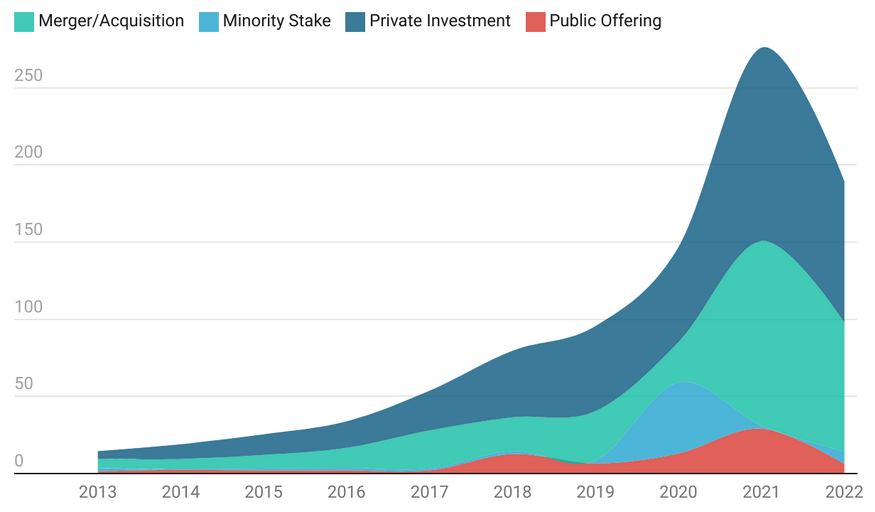
\includegraphics[width=\textwidth]{ai-investement.png}
    \caption{Inversión global en IA en miles de millones \cite{Letzing2024-nn}.}
    \label{fig:ai-investement}
\end{figure}

Nos encontramos en un momento en el que la demanda de equipos cualificados 
que puedan hacer frente a los nuevos desafíos es mayor que nunca. La complejidad
de los proyectos de IA también está en aumento, ya que las aplicaciones de IA
se vuelven más sofisticadas, abarcan una gama más amplia de funciones, requieren
un mayor número de datos y los modelos se vuelven cada vez más complejos. Esta
situación a forzado a las empresas a buscar nuevas formas de gestionar sus proyectos
que han llevado a la creación de nuevas metodologías, adaptadas a las necesidades
a los nuevos retos que se presentan. Si bien es cierto que mucha información es
compartida con la comunidad, existe un gran secretismo en torno a la forma de operar
de las empresas más grandes, lo que dificulta la adopción de estas metodologías.
Podemos resaltar positivamente el caso de Meta \cite{metaia}, que es el mayor 
referente en cuanto contribución y apertura de sus desarrollos en IA.\medskip

Por todo ello, es necesario realizar contribuciones que se centren en el como 
se debería operar dentro de un equipo. Se requiere de una referencia clara sobre las 
directrices que se deben aplicar para poder implementar un estándar tecnológico y
operacional dentro de un grupo de trabajo, así como las herramientas, metodologías y buenas prácticas
a seguir para hacer un uso eficiente de los recursos y obtener resultados de calidad.
Este documento representa un estándar que se ha aplicado en base a unas necesidades
concretas y, aunque no está pensado para poder ser adoptado de forma literal por otros equipos,
se muestra el camino que se ha seguido desde la adopción de plataformas MLOps hasta la creación
de un sistema de conocimiento para la reutilización de trabajo. La justificación de este
documento es exponer el trabajo realizado y servir como referencia equipos que quieran implementar
un estándar similar o busquen inspiración para crear el suyo propio.
 
%% Antecedentes -> Contenido general
%% Estado del arte -> Contribuciones de otros equipos
%% Referencias sobre replicabilidad 

\subsection{Antecedentes}
En la sección de antecedentes, se profundiza en aquellos conceptos esenciales que son 
indispensables para entender el alcance y las contribuciones de este trabajo, así como 
para situarlo dentro de un marco conceptual adecuado. Se abordan aspectos fundamentales 
que no solo proporcionan contexto, sino que también establecen las bases teóricas y 
metodológicas sobre las cuales se construye la investigación.

\subsubsection{Diseño Atómico}
El diseño atómico es una metodología de diseño que se centra en la creación
de sistemas modulares y reutilizables. La idea principal es dividir
las diferentes funcionalidades de un sistemas en sus partes más fundamentales,
de manera que cada una de estas partes pueda ser reutilizada en diferentes
contextos. Este enfoque permite tener un mayor control sobre cada una de las
partes del sistema, facilitando su mantenimiento, documentación y reutilización.
Originalmente, el diseño atómico ha sido aplicado en el diseño de interfaces
de usuario, pero su filosofía puede ser aplicada a cualquier sistema de diseño
modular. En el contexto de este proyecto, el diseño atómico se aplicará al
diseño de un sistema de componentes para el desarrollo de modelos de aprendizaje
automático.\medskip

Dentro del diseño atómico, los componentes se dividen en cinco categorías
principales, que representan diferentes niveles de abstracción. Estas categorías
son: átomos, moléculas, organismos, plantillas y páginas. Cada una de estas
categorías representa un nivel de abstracción diferente, y se relaciona con
las demás categorías de manera jerárquica. La figura \ref{fig:atomic-design}
muestra la estructura conceptual del diseño atómico. 

\begin{figure}[ht]
    \centering
    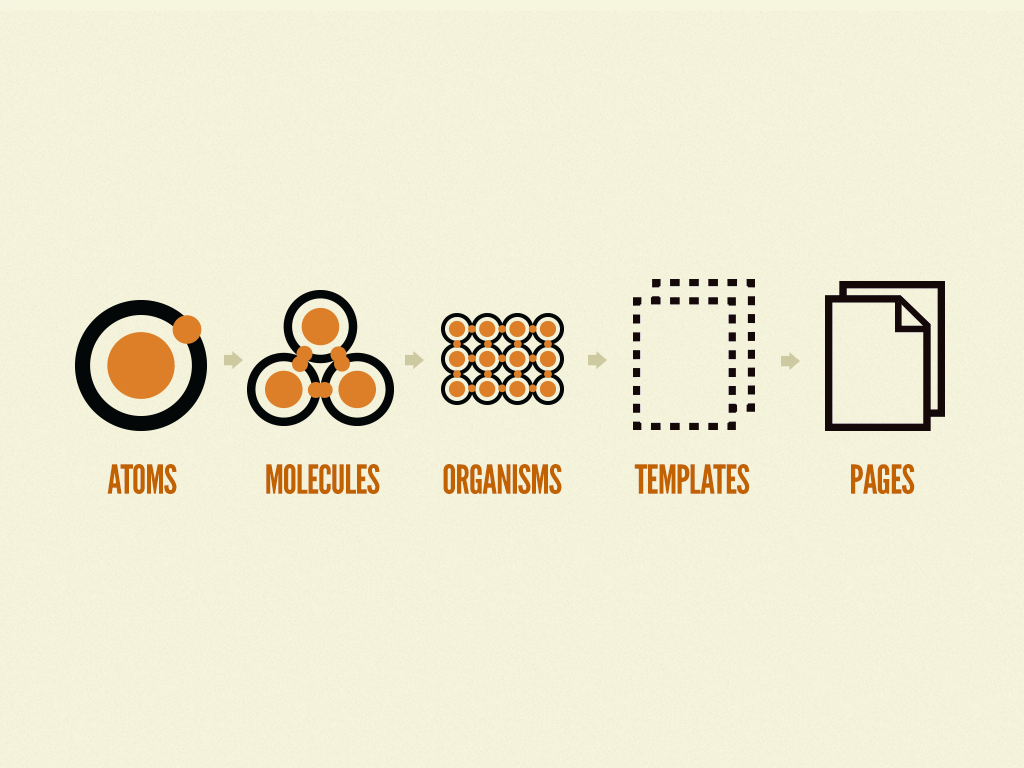
\includegraphics[width=0.7\textwidth]{atomic-design-process.png}
    \caption{Estructura conceptual diseño atómico \cite{frost2016atomic}.}\label{fig:atomic-design}
\end{figure}

A continuación, se describen brevemente cada una de las categorías:
\begin{itemize}
    \item \textbf{Átomos:} Los átomos son los componentes más básicos de un sistema
    de diseño. Representan las funcionalidades más fundamentales, solo tienen
    una responsabilidad y no dependen de otros componentes.
    \item \textbf{Moléculas:} Las moléculas son la combinación de varios átomos
    para formar una funcionalidad más compleja. Representan la combinación de
    diferentes funcionalidades básicas para formar una funcionalidad más compleja.
    \item \textbf{Organismos:} Los organismos son la combinación de varias moléculas
    y átomos para formar una funcionalidad completa.
    \item \textbf{Plantillas:} Las plantillas son la combinación de varios Organismos
    para dar forma a un contenido.
    \item \textbf{Páginas:} Las páginas son la combinación de varias plantillas.
\end{itemize}

Esta estructura jerárquica permite que los componentes sean reutilizados en
diferentes contextos, y que cada uno de ellos pueda ser modificado de manera
independiente. Además, se facilita la documentación y el mantenimiento de los
componentes, ya que cada uno de ellos es independiente de los demás. Podemos
ver multitud de ejemplos de diseño atómico en grandes empresas y que nosotros utilizamos
a diario, como por ejemplo en la creación de sistemas de diseño Microsoft Fluent
Design o Google Material Design entre otros.\medskip

Aunque el diseño atómico se ha aplicado tradicionalmente a la creación de interfaces
de usuario, su filosofía puede ser aplicada a cualquier sistema de diseño modular.
En el contexto de este proyecto, el diseño atómico se aplicará para la creación de un
sistema de componentes en el desarrollo de modelos de aprendizaje automático.
Traeremos la filosofía del diseño atómico y la adaptaremos a nuestro contexto,
con las particularidades y necesidades que requiere el desarrollo de modelos de
aprendizaje automático. 

\subsubsection{Machine Learning Operations (MLOps)}
El desarrollo de modelos de aprendizaje automático es un proceso complejo que implica
la recopilación de datos, la creación de modelos, la evaluación de los modelos y su
puesta en producción. Cada una de estas etapas requiere de diferentes herramientas y
prácticas, y es importante que estas herramientas y prácticas estén integradas de manera
coherente para garantizar la eficacia del proceso. Los principios de MLOPs son una serie de prácticas y herramientas que se utilizan
para gestionar el ciclo de vida de los modelos de aprendizaje automático. Como se muestra en la
figura \ref{fig:mlops-workflow}, este enfoque busca aplicar las mejores tendencias dentro de la 
ingeniería de software al desarrollo de modelos, con el objetivo de mejorar la eficiencia, la 
calidad y la escalabilidad.\medskip

\begin{figure}[ht]
    \centering
    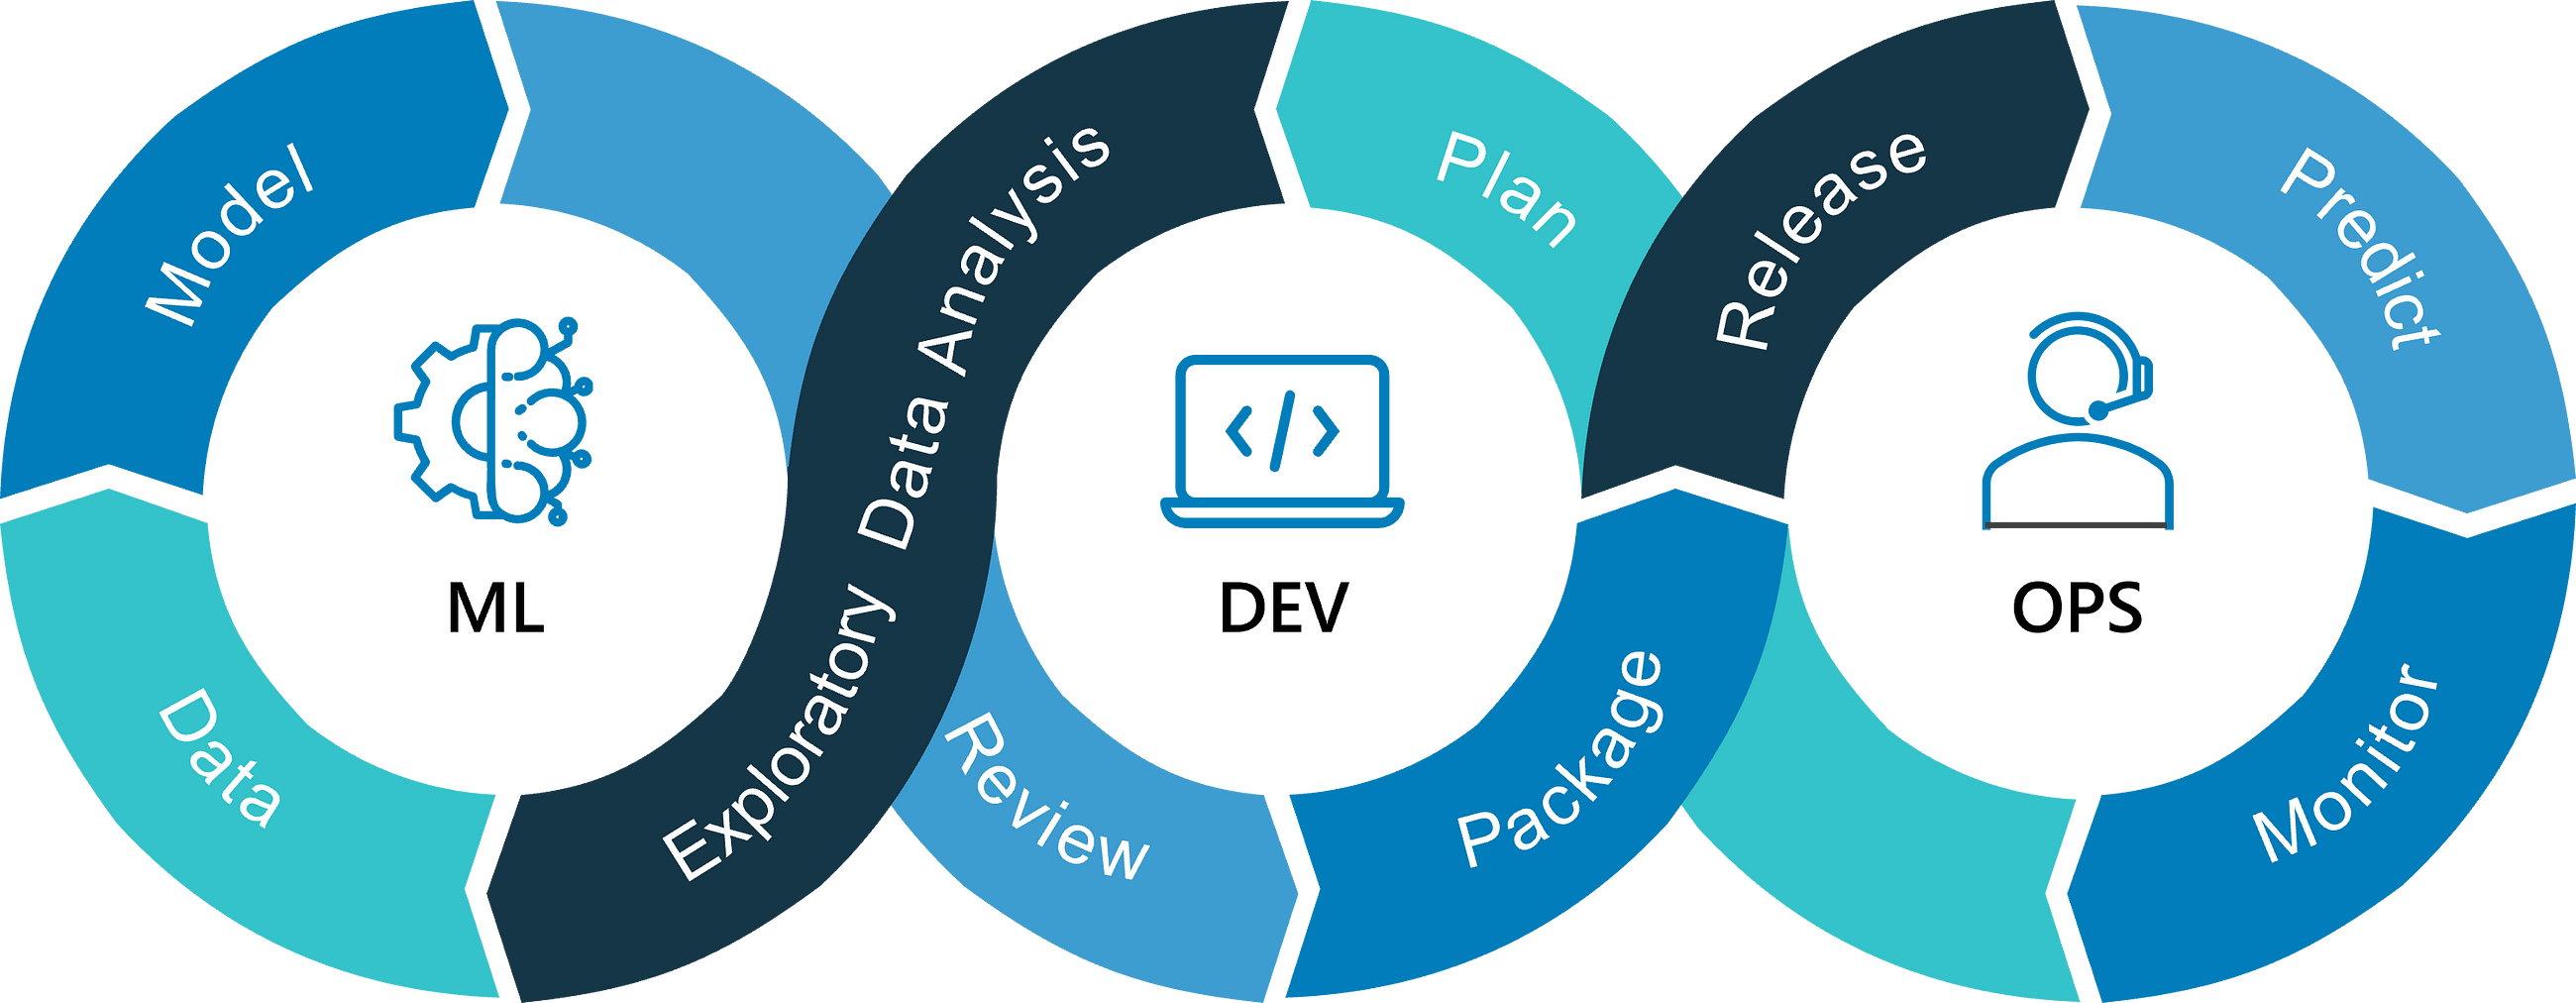
\includegraphics[width=\textwidth]{mlops-workflow.png}
    \caption{Ciclo de vida MLOps}\label{fig:mlops-workflow}
\end{figure}


Algunos de los principios clave de MLOps son:

\begin{itemize}
    \item \textbf{Automatización:} la automatización es esencial para mejorar la eficiencia del
    desarrollo de modelos y prevenir errores. Esto implica automatizar tareas como la 
    generación de datos, el despliegue de modelos, evaluación y su puesta en producción.
    \item \textbf{Colaboración y reproducibilidad:} uno de los desafíos en el Aprendizaje Automático es lograr 
    reproducir resultados de manera consistente, dada la naturaleza aleatoria de los algoritmos.
    MLOps busca, en la medida de lo posible, garantizar cierta consistencia entre los resultados
    obtenidos durante diferentes ejecuciones de un modelo para facilitar la colaboración entre
    los miembros del equipo.
    \item \textbf{Monitorización:} una vez que un modelo está en producción, es importante monitorizar
    su rendimiento para garantizar su eficacia y detectar posibles problemas. La monitorización
    permite crear alertas en caso de que el modelo no funcione correctamente y tomar medidas
    para corregirlo como por ejemplo, actualizar el modelo con nuevos datos.
    \item \textbf{Gestión de versiones:} controlar las versiones de los modelos y los datos es esencial
    para garantizar la reproducibilidad y la trazabilidad de los modelos. La gestión de versiones
    permite a los equipos comprender cómo ha evolucionado un modelo a lo largo del tiempo e incluso
    retroceder a versiones anteriores fuera necesario.
\end{itemize}

\subsection{Estado del arte}
La sección de estado del arte se centra en recopilar información sobre las tendencias
actuales dentro del ámbito del aprendizaje automático y la inteligencia artificial.
Debido a la diversidad de ramas que abarca la creación de un estándar tecnológico y
operacional, se han seleccionado aquellas que se consideran más relevantes o presentan
un mayor peso en cuanto a la toma de decisiones.

\subsubsection{Irrupción de las metodologías ágiles}
La aparición de metodologías ágiles en el desarrollo de software, con sus numerosas ventajas, 
ha dejado en desuso muchas metodologías clásicas. Las metodologías ágiles introdujeron el 
concepto de DevOps como un cambio de mentalidad \cite{salvucci2021mlops} 
en la que los diferentes equipos colaboran para implementar procesos más rápidos y 
entregar nuevas funcionalidades al cliente de manera más ágil. MLOps es una extensión de 
DevOps que ha surgido muy recientemente y, por lo tanto, existen pocos estudios que 
aborden el tema \cite{kreuzberger2022mlops}\cite{recupito2022multivocal}.\medskip

Principalmente existen dos formas para implementar MLOps en una organización, uno es
a través de los sistemas cloud que ofrecen servicios MLOps como Azure ML \cite{microsoft2023azureml}, 
AWS Sagemaker \cite{aws_sagemaker} o Google Cloud Vertex AI \cite{google2023vertexai}. El otro es a través del despliegue de una plataforma open source
como MLFlow dentro de la infraestructura propia. Las principales diferencias entre ambas
opciones son el coste y la flexibilidad, ya que los servicios cloud ofrecen una mayor
facilidad de uso y mejor experiencia de desarrollo, pero a un coste mayor. Por otro lado,
la implementación de una plataforma open source requiere de un mayor esfuerzo pero ofrece
se recompensa con una mayor flexibilidad y control sobre la infraestructura.

\subsubsection{Problemas de replicabilidad}
La crisis de replicabilidad es un fenómeno crítico en la comunidad científica,  
donde los resultados de los estudios a menudo no pueden replicarse con nuevos datos \cite{puetz2024replication}.
Este problema es muy destacado en numerosos campos científicos, que se han enfatizado particularmente 
en disciplinas como la psicología, la salud y la medicina \cite{puetz2024replication}\cite{Baker_2016}, donde hallazgos incorrectos 
podrían tener consecuencias graves. Durante los últimos años, la crisis de replicabilidad ha
sido objeto de debate dentro de la rama de la inteligencia artificial, donde la falta de
transparencia, la complejidad de los modelos y la imposibilidad de replicar los resultados
han sido identificados como problemas clave.

\begin{figure}[ht]
    \centering
    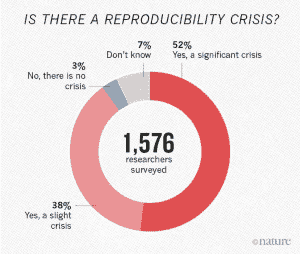
\includegraphics[width=0.75\textwidth]{crisis-survey.png}
    \caption{Encuesta a 1500 investigador sobre la reproducibilidad en la ciencia \cite{Baker_2016}}\label{fig:crisis-survey}
\end{figure}

La confusión se ve incrementada por el uso variado de términos clave como reproducibilidad, 
replicabilidad y repetibilidad, \cite{readytensor} dificultando los esfuerzos para abordar estos problemas de 
manera efectiva. Se definen los diferentes términos de la siguiente manera:
\begin{itemize}
    \item \textbf{Repetibilidad:} se centra en la consistencia de los resultados de la investigación cuando el equipo 
    original re-ejecuta su experimento bajo condiciones inalteradas. 
    \item \textbf {Reproducibilidad:} se logra cuando investigadores independientes validan los hallazgos del 
    experimento original empleando el documentado original. Esta validación puede ser directa, utilizando 
    los datos y el código originales, o independiente, a través de la reimplementación del experimento, 
    probando así la fiabilidad de los resultados en diferentes equipos.
\end{itemize}

Una serie de estudios y encuestas subrayan la gravedad de la situación \cite{Baker_2016}.
Como se muestra en la figura \ref{fig:crisis-survey}, una encuesta realizada a 1500 investigadores
encontró que el 50\% de ellos afirman que que hay una crisis significativa y un 40\% que hay
una crisis moderada, dejando solo un 10\% que no ve una crisis en la replicabilidad de los estudios.
Existen multitud de casos donde los intentos de volver a ejecutar experimentos dan como resultado 
a una amplia desviación, incluso bajo condiciones idénticas\ref{fig:crisis-survey}.
Los propios investigadores tienen dificultades para reproducir sus propios experimentos.
La figura \ref{fig:self-reproduce} nos da una idea de lo frecuente que es este problema,
donde en el caso de la física e ingeniería, el 50\% de los encuestados han tenido problemas
reproduciendo sus experimentos, lo que se ve reflejado en que el 70\% de ellos haya tenido
problemas al intentar reproducir los experimentos de otros investigadores.

\begin{figure}[ht]
    \centering
    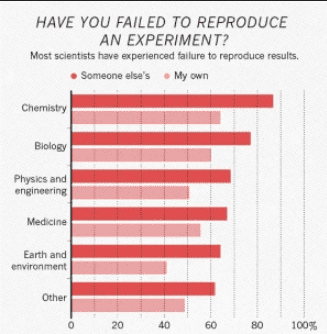
\includegraphics[width=\textwidth]{self-reproduce.png}
    \caption{Problemas con la reproducibilidad por disciplina \cite{Baker_2016}}\label{fig:self-reproduce}
\end{figure}

Estos problemas se consideran como los principales causantes como se puede ver en la figura \ref{fig:repro-factor}.
Factores como la falta de información sobre detalles experimentales y los tiempos de publicación, enfatizando 
la necesidad urgente de un enfoque más sistemático y transparente. Sin contar los problemas
directamente relacionados con el desarrollo, como son la procedencia y calidad de los datos, la 
elección del algoritmo, el hardware utilizado para su entrenamiento, el preprocesamiento de 
los datos, entre otros.

\begin{figure}[ht]
    \centering
    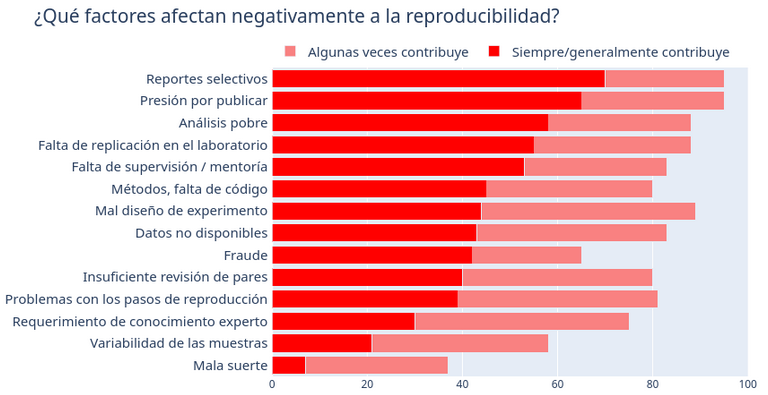
\includegraphics[width=0.5\textwidth]{repro-factor.png}
    \caption{Factores que contribuyen a la irrepoducibilidad \cite{Baker_2016}}\label{fig:repro-factor}
\end{figure}

Aunque la crisis de un problema complejo y multifacético, existen
algunas medidas que pueden tomarse para abordarlo. Algunas de estas medidas que encontramos
en al literatura son un mejor supervisión, mejora del proceso de validación, incentivar
buenas practicas de desarrollo, entre otras

\subsubsection{Calidad del software y buenas prácticas}


\pagebreak
    \section{Objetivos y alcance}
En esta sección se introducen los objetivos del 
proyecto, habiéndose realizado una division entre el principal y los
secundarios. Ademas de ello, se presentan los elementos que forman el alcance,
asi como se comentan otros que no.

\subsection{Objetivos generales}
El objetivo principal del proyecto es diseñar e implementar un estándar tecnológico y 
operacional que cubra las necesidades más comunes dentro de un equipo de \textit{data science}. Se 
busca agilizar los tiempos de desarrollo y estandarizar los procesos, con el fin de
facilitar la colaboración entre investigadores y la reutilización del conocimiento. A
continuación, se detallan los objetivos específicos que guiarán el desarrollo:

\begin{itemize}
    \item \textbf{Agilizar el proceso inicial de proyectos:} Optimizar las primeras etapas 
    de los proyectos, identificando y eliminando aquellos procesos repetitivos que no aportan
    valor y que puedan retrasar su puesta en marcha. 
    \item \textbf{Facilitar la colaboración entre investigadores:} Implementar herramientas y 
    métodos que fomenten una cooperación fluida y efectiva entre los miembros del equipo de 
    investigación, con el fin de potenciar la sinergia y aprovechar al máximo el conocimiento 
    colectivo.
    \item \textbf{Definir procesos mediante buenas prácticas:} Establecer un marco de trabajo 
    basado en buenas prácticas de gestión de proyectos, con el objetivo de estandarizar los 
    procesos y garantizar su eficiencia y calidad.
    \item \textbf{Automatizar el desarrollo de modelos robustos:} Investigar y aplicar 
    técnicas que contribuyan al desarrollo automático de modelos de aprendizaje automático,
    con el fin de reducir el tiempo y el esfuerzo necesarios para obtener resultados de calidad.
    \item \textbf{Promover la reutilización del conocimiento:} Desarrollar mecanismos y herramientas 
    que faciliten la captura, organización y difusión del conocimiento generado durante el desarrollo 
    de los proyectos, con el propósito de fomentar su reutilización en futuras investigaciones y 
    actividades relacionadas.
\end{itemize}

El cumplimiento de estos objetivos se espera que no solo mejore la eficiencia y la calidad de los 
proyectos, sino que también contribuya a la creación de un entorno de trabajo más colaborativo y
enriquecedor para los miembros del equipo de investigación.

\subsection{Alcance}
En esta sección se definen los límites del proyecto, estableciendo lo que está
incluido y excluido dentro mismo. Se describirá de manera detallada las
actividades que forman parte del desarrollo final, así como aquellos elementos
que no están incluidos en el alcance del proyecto. Aunque el enfoque de este 
proyecto podría aplicarse a una amplia variedad de problemas en el ámbito del 
aprendizaje automático, en el contexto de este TFM nos centraremos en tres de 
los casos más comunes dentro del marco de las series temporales: Forecasting, 
Clasificación y Detección de Anomalías. A continuación, se detallan las 
actividades que forman parte del alcance del proyecto.

\subsubsection{Dentro del alcance}
\begin{itemize}
    \item \textbf{Integración de sistemas externos:} Se incluirá la configuración de sistemas 
    externos, como plataformas MLOPs o herramientas de visualización, con las plantillas 
    de proyectos base. Esto permitirá una integración más fluida y rápida de estos sistemas con 
    los proyectos, facilitando el flujo de datos y la visualización de resultados.
    \item \textbf{Plantillas de proyectos base:} Desarrollar plantillas para 
    los tres problemas de series temporales comentados anteriormente. Estas plantillas 
    servirán como punto de partida para proyectos específicos dentro de cada uno de estos dominios
    y definirán desde el principio una estructura y un conjunto de herramientas comunes. Además,
    se incluirán ejemplos de código y documentación que faciliten su uso y comprensión.
    \item \textbf{Componentes esenciales:} Identificar y almacenar los componentes 
    esenciales de cada proyecto, incluyendo modelos, algoritmos, métricas de evaluación y
    preprocesamiento de datos. Estos componentes se almacenarán y documentarán de forma
    que puedan ser reutilizados en futuros proyectos, facilitando la transferencia de conocimiento.
    \item \textbf{Proceso de AutoML:} Diseñará y ejecutar procesos de AutoML 
    (Machine Learning Automatizado) que demostrará cómo se pueden combinar los conocimientos 
    adquiridos de todos los proyectos para desarrollar un sistema de aprendizaje automático 
    automatizado. Este proceso utilizará las plantillas y componentes esenciales almacenados 
    para generar modelos de forma automática.
\end{itemize}

\subsubsection{Fuera del alcance}
\begin{itemize}
    \item \textbf{Desarrollo de modelos específicos:} Aunque se incluirán ejemplos de
    modelos y algoritmos, el desarrollo de modelos específicos para problemas concretos
    no forma parte del alcance de este proyecto. Se espera que los modelos desarrollados
    sean generales y puedan ser adaptados a problemas específicos por los usuarios.
    \item \textbf{Despliegue de modelos:} El despliegue de modelos en producción no forma
    parte del alcance de este proyecto. Se espera que los modelos desarrollados puedan ser
    desplegados en sistemas de producción, pero no se incluirá en este proyecto. El enfoque
    se centrará exclusivamente en el desarrollo de los mismos.
\end{itemize}

\pagebreak
    \section{Metodología del Proyecto}
En esta sección, se describirá la metodología para abordar tanto el
desarrollo del software como la propia metodología de investigación. La metodología
de desarrollo de software se basa en el uso de metodologías ágiles \cite{Agile_Microsoft}, concretamente
en la metodología Scrum \cite{Atlassian_Scrum}. Por otro lado, la metodología de investigación es una
metodología propia diseñada para abordar problemas dentro del marco de trabajo de
los problemas combinatorios NP-Hard diseñada por el autor de este trabajo. Esta
metodología se basa en el uso de técnicas de IL.

\pagebreak 
    \section{Desarrollo del Proyecto}
En esta sección se detallan los aspectos más relevantes del desarrollo del proyecto.
Se profundizará en los diferentes aspectos del diseño, la implementación y la
prueba de los sistemas y componentes desarrollados. Además, se describirán las
herramientas y tecnologías utilizadas, así como los procesos y metodologías
empleadas para el desarrollo del proyecto. A continuación, se muestra una vista general de los diferentes elementos
que conforman la estructura del marco de trabajo.

\begin{figure}[ht]
    \centering
    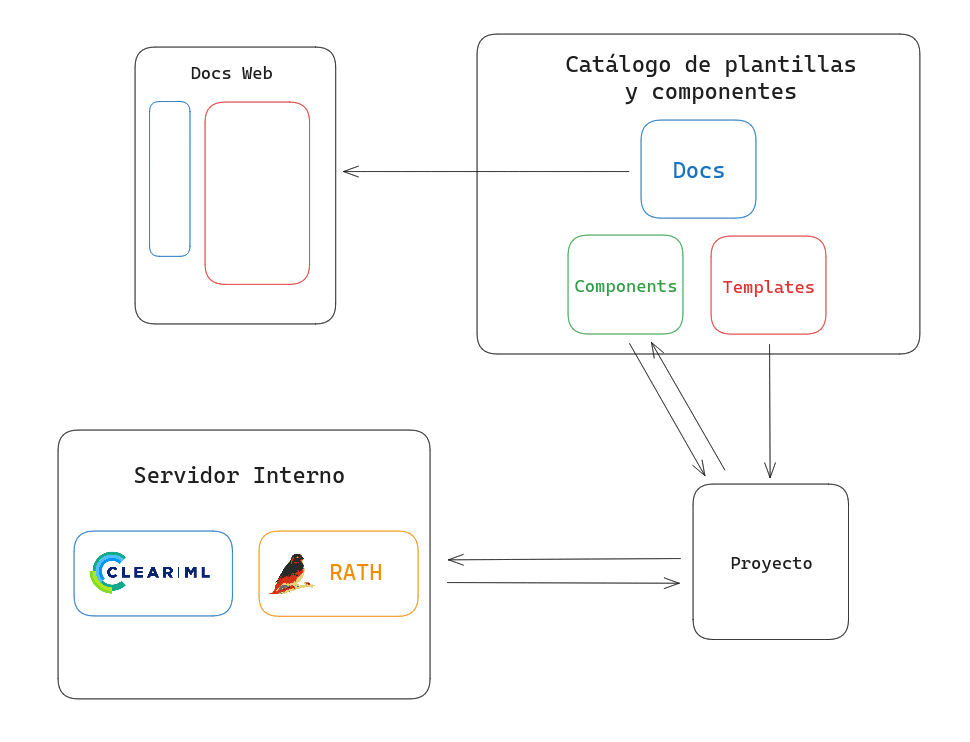
\includegraphics[width=\textwidth]{general-vision.png}
    \caption{Vista general del proyecto}\label{fig:general-vision}
\end{figure}

Dentro de la estructura general del proyecto, se pueden identificar tres elementos
principales: la infraestructura y herramientas, el catálogo de componentes y la
documentación del proyecto. Cada uno de estos elementos se encarga de aspectos
diferentes dentro del ecosistema del proyecto, y se relacionan entre sí para formar
un sistema completo. La idea principal es que la infraestructura sea complementaria
al desarrollo, estando al alcance de los investigadores de una forma sencilla. El catálogo
de componentes y plantillas se encarga de proporcionar una base sólida sobre la que
construir los diferentes proyectos, automatizando la creación de proyectos siguiendo 
las mejores prácticas y proporcionando una base sólida sobre la que construir. Por último,
la documentación del proyecto se encarga de proporcionar una guía clara y detallada
sobre el uso de las herramientas y componentes, así como de los procesos y metodologías
empleadas en el desarrollo del proyecto.

\subsection{Infraestructura y herramientas}
\subsubsection{Descripción general de la infraestructura}
La infraestructura y las herramientas son la base sobre la que se construirán
los diferentes proyectos de aprendizaje automático. Se encargan de proporcionar
un entorno de desarrollo e investigación eficiente, que permita a los miembros
del equipo centrarse en el desarrollo de modelos sin tener que preocuparse por
la configuración. Concretamente, se han desplegado dos plataformas 
que vienen a cubrir varias de las necesidades fundamentales de los proyectos
como son la gestión y exploración de datasets, la monitorización de experimentos o
el almacenamiento de modelos de inteligencia artificial. Además, se ha añadido un sistema de autenticación 
para garantizar la seguridad y privacidad de los datos.\medskip

Esta infraestructura se ha desplegado en un servidor interno de la empresa
utilizando contenedores de Docker. La elección de esta tecnología se debe a
que permite la creación de entornos aislados y portables, lo que facilita el
despliegue de las aplicaciones. Se ha utilizado Docker Compose para
sincronizar el despliegue de los diferentes servicios, lo que permite
realizar despliegues automatizados mediante las acciones de GitLab CI. La
figura \ref{fig:internal-server} muestra una vista general de la infraestructura
desplegada en el servidor interno de la empresa, donde se pueden observar
como se integran los diferentes servicios y sus respectivas conexiones. Además,
se puede observar que todos los servicios están interconectados mediante un
proxy inverso mediante Nginx, que se encarga de redirigir las peticiones en 
función de la URL. Esto permite que todos los servicios sean
accesibles desde el exterior a través de un único punto de entrada y que el
sistema de autenticación sea común para todos ellos.

\begin{figure}[ht]
    \centering
    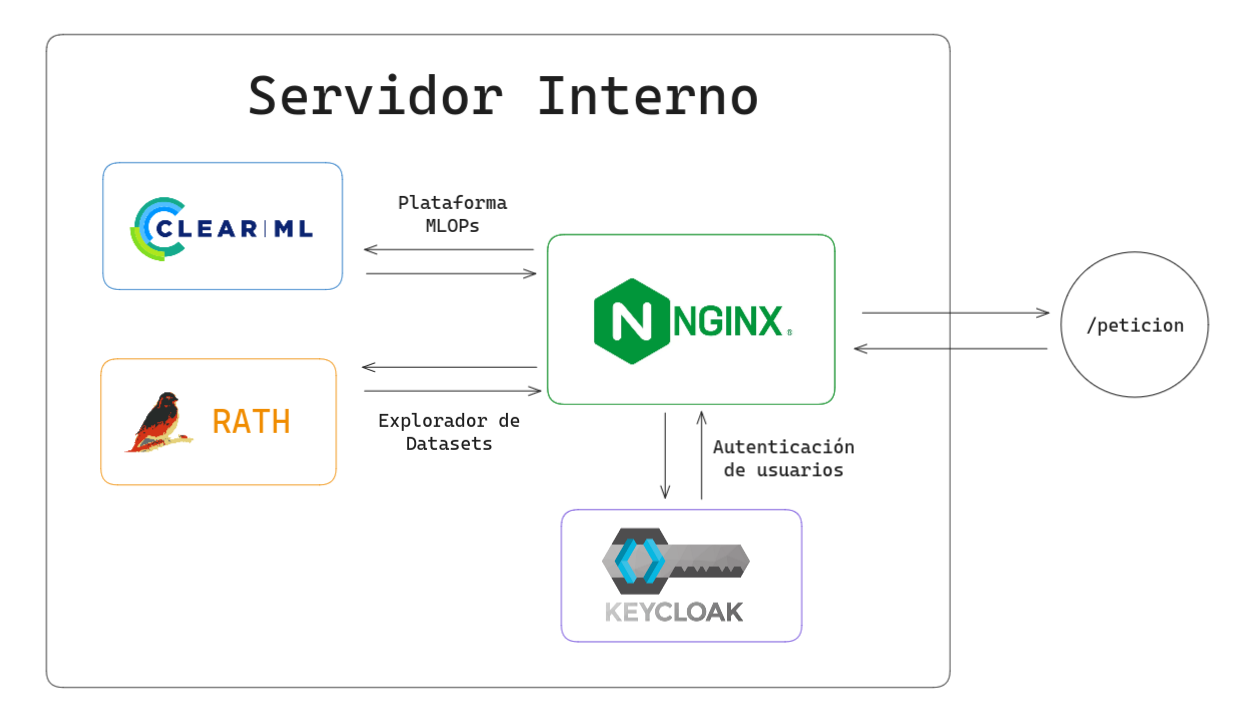
\includegraphics[width=\textwidth]{internal-server.png}
    \caption{Vista general del proyecto}\label{fig:internal-server}
\end{figure}

\subsubsection{Selección de plataformas}
Previo a la elección de las plataformas integradas, se realizó una evaluación
a nivel de equipo para determinar las necesidades que se debían cubrir. Se
identificaron las siguientes funcionalidades fundamentales:

\begin{itemize}
    \item \textbf{F1:} Versionado y almacenamiento de dataset.
    \item \textbf{F2:} Monitorización de experimentos.
    \item \textbf{F3:} Almacenamiento de modelos de inteligencia artificial.
    \item \textbf{F4:} Integración de métricas en datasets y visualización de resultados.
    \item \textbf{F5:} Exploración de datasets.
\end{itemize}

Una vez identificadas las necesidades, se consensuó un criterio de selección
para las plataformas integradas. Este criterio es un criterio de mínimos, es
decir, se seleccionarán las plataformas que cumplan con el criterio mínimo
establecido y que, además, ofrezcan funcionalidades adicionales que puedan
ser de utilidad para el equipo. El criterio de selección se basa en los
siguientes aspectos: 

\begin{itemize}
    \item \textbf{C1 (Facilidad de uso):} Se valora muy positivamente la facilidad de uso de las
    plataformas, ya que se considera que no todo el equipo no tiene experiencia
    previa en el uso de estas herramientas.
    \item \textbf{C2 (Integración con otras herramientas):} Es fundamental que las
    plataformas integradas sean compatibles con las librerías y herramientas
    que se utilizan generalmente en proyectos (TensorFlow, PyTorch, etc.).
    \item \textbf{C3 (Poca dependencia sobre la infraestructura):} Medimos la dependencia
    sobre una plataforma como el numero de acciones que se deben realizar para
    migrar un proyecto vanilla, es decir, un proyecto que no ha sido
    desarrollado con la plataforma en mente. Y penalizando aquellas practicas
    que sean propias de la plataforma y que no sean comunes en la industria.
\end{itemize}

Con estos criterios en mente, se tuvieron en cuenta las siguientes
plataformas a la hora de realizar la evaluación: MLflow, ClearML, Kedro, ZenML, Data Version Controller (DVC),
Rath, Apache Superset. Cada una de estas plataformas tiene diferentes enfoques y 
funcionalidades, pero todas ellas cubren una o varias de las necesidades fundamentales
identificadas, por lo que se consideraron candidatas para su integración en la
infraestructura. La infraestructura final se compondrá de una o varias de estas
plataformas en función de los criterios previamente establecidos. A continuación, se 
muestra un análisis detallado de las plataformas evaluadas y las funcionalidades que ofrecen.

\begin{itemize}
    \item \textbf{MLflow:} MLflow es una plataforma MLOPs de código abierto para la gestión del ciclo de vida de
    los modelos. Ofrece una interfaz de usuario para el seguimiento de experimentos, la gestión de modelos 
    y la implementación de modelos en diferentes entornos. MLflow es compatible con la mayor parte de librerías de aprendizaje 
    automático, como TensorFlow o PyTorch. Uno de los puntos fuertes de MLflow es su gran comunidad, ya que es
    una de las plataformas más utilizadas en la industria. Sin embargo, no ofrece funcionalidades relacionadas con
    la gestión, evaluación o versionado de datasets ni con la exploración de los mismos. La dependencia sobre la
    plataforma varía en función de la tarea que se quiera realizar, pero en general, es una plataforma que no
    ata al usuario a su ella. La documentación se queda corta en cuestión de claridad y ejemplos, lo que puede
    dificultar la adopción de la plataforma por parte de los miembros del equipo.
    \item \textbf{ClearML:} ClearML al igual que MLflow, es una plataforma MLOps de código abierto que ofrece
    las mismas funcionalidades que MLflow en relación a la gestión a la gestión de experimentos, pero con la
    diferencias, que este si cuenta con funcionalidades relacionadas con la gestión, evaluación o versionado de
    datasets. ClearML también es compatible con la mayor parte de librerías populares aunque no tantas ni tan
    variadas como MLflow, pero ofrece una API que permite de la integración de estas de forma manual. La
    dependencia sobre la plataforma es mínima, ya que con pocos cambios se pueden lanzar experimentos sobre
    un código base. La documentación es clara y ofrece ejemplos en formato tanto de texto como de video, con
    proyectos sencillos y claros que permiten entender rápidamente el funcionamiento de la plataforma. El 
    principal punto débil de ClearML es que no cuenta con una gran comunidad, lo que puede dificultar a
    la hora de encontrar soluciones a ciertas problemáticas. Otro de sus puntos débiles es que por defecto
    no cuenta con un sistema de autenticación robusto, lo que te obliga a implementar uno por tu cuenta.
    \item \textbf{Data Version Controller (DVC):} DVC y DVC Studio son dos herramientas de código abierto que
    están diseñadas para manejar grandes volúmenes de datos, modelos y experimentos. DVC
    se centra en el versionado y almacenamiento de datasets, mientras que DVC Studio se centra en la
    monitorización de experimentos, visualización de resultados y almacenamiento de modelos. Además, 
    DVC Live proporciona integraciones con un número considerable de librerías de aprendizaje automático.
    La documentación está bien estructurada aunque no es tan clara como la de ClearML, pero cuenta con una
    comunidad bastante activa. En cuanto a los aspectos negativos de DVC, la principal desventaja es que
    la curva de aprendizaje es bastante pronunciada, lo que dificulta su adopción. Otro punto en contra
    es la dependencia gigantesca que tienen los proyectos que usan DVC, ya que se necesita de muchos archivos
    de configuración, integraciones manuales dentro del código y un dominio completo de los comandos de la
    herramienta para poder trabajar con ella.
    \item \textbf{Kedro:} TODO:
    \item \textbf{ZenML:} ZenMl es una plataforma de código abierto encargado de la orquestación de pipelines en
    proyectos de aprendizaje automático. Ofrece una experiencia de desarrollo cómoda y modular, que facilita
    la reutilización de código. Además, ZenML cuenta con integraciones para las platformas de almacenamiento
    mas populares, como AWS y Google Cloud. A diferencia de ClearMl y MLflow, este no está enfocado en la
    gestión de experimentos ya que no es una plataforma MLOps, aunque si que ofrece conexiones con estas
    para poder redireccionar nuestros experimentos. La documentación es clara y podemos encontrar diversos repositorios 
    con ejemplos de uso o integración con otras herramientas. El problema de esta radica principalmente
    en el hecho de que al no ser una plataforma MLOps, no ofrece funcionalidades relacionadas con la gestión
    o versionado de datasets, lo que es un punto negativo para nuestro caso de uso. Otro de los problemas
    es que las plataformas con las que ofrece integración no comparten las mismas credenciales dentro de su capa
    gratuita, lo que dificulta en gran medida su uso. Además, dentro de la capa gratuita estas plataformas 
    funcionan de forma independiente, lo que vuelve muy complicado el trabajo con ellas.
    Por último, la funcionalidad de orquestación de pipelines también viene incluida en ClearML, por lo que
    no aporta ninguna funcionalidad adicional que no este cubierta.
    \item \textbf{Rath:} herramienta de exploración de datasets que permite una exploración semi-automática
    de datasets. Muy fácil de utilizar, ya que cuenta con un modo copilot que te sugiere diferentes gráficos
    y estadísticas en función de los datos que estés explorando. Además, no requiere de ninguna configuración
    previa, ya que se puede utilizar directamente desde el navegador.
    \item \textbf{Apache Superset:} Apache Superset es una plataforma de visualización de datos de código abierto 
    que ofrece una amplia gama de características para explorar y visualizar datos de manera interactiva. Con una 
    interfaz intuitiva y basada en web, Superset permite a los usuarios crear paneles de control, gráficos y tablas 
    dinámicas con facilidad. Además, ofrece integraciones con diversas fuentes de datos y admite la creación de 
    paneles de control en tiempo real. Una de las fortalezas de Apache Superset es su comunidad activa y en constante 
    crecimiento, lo que garantiza un soporte sólido y una mejora continua de la plataforma. Sin embargo, la integración
    con el resto de herramientas es limitada, ya que el propio Superset requiere de un formato de datos concreto para
    poder subir los datos a la plataforma, lo que puede dificultar su integración y generar duplicidad en cuanto a los
    datos almacenados, ya que se necesitaría una copia de los datos en el formato que requiere Superset. Nuestro objetivo
    es que esta herramienta agilice el proceso de exploración de datos, por lo que no es una opción viable por el momento.
    \item \textbf{Grafana:} Grafana es una plataforma de análisis y visualización de métricas de código abierto que 
    se ha convertido en una opción popular para monitorear sistemas y aplicaciones. Con una amplia gama de complementos 
    y paneles personalizables, Grafana permite a los usuarios crear cuadros de mando y gráficos altamente personalizados 
    para visualizar datos de diferentes fuentes. Además, ofrece características avanzadas como alertas, anotaciones y 
    exploración de datos en tiempo real. Grafana es altamente modular y extensible, lo que facilita su integración con 
    diversas tecnologías y sistemas de monitoreo. El problema de Grafana es el mismo que el de Superset, ya que requiere
    de un formato de datos concreto para poder subir los datos a la plataforma, lo que puede dificultar su integración y
    generar duplicidad en cuanto a los datos almacenados. Además, de su curva de aprendizaje, que es bastante pronunciada.
\end{itemize}

\begin{table}[ht]
    \centering 
    \begin{tabular}{lccccccccc}  
        
        \toprule
        \multirow{2}{*}{\parbox[c]{.2\linewidth}{\centering Tecnología}} & 
        \multicolumn{5}{c}{\textbf{Funcionalidades}} && 
        \multicolumn{3}{c}{\textbf{Criterios}} \\ 
        
        \cmidrule{2-6} \cmidrule{8-10}
        & {\centering F1} & {F2} & {F3}& {F4} & {F5} && {C1} & {C2} & {C3}\\
        
        \midrule
        MLflow           & --     & \check & \check & --     & --     && \check & \check & \check \\
        ClearML          & \check & \check & \check & \check & --     && \check & \check & \check \\
        DVC              & \check & \check & \check & \check & --     && --     & \check & --     \\ 
        Kedro            & --     & \check & \check & --     & --     && \check & \check & \check \\  
        ZenML            & --     & --     & --     & --     & --     && --     & --     & --     \\ 
        Rath             & --     & --     & --     & --     & \check && \check & --     & \check \\ 
        Apache Superset  & \check & --     & --     & \check & --     && --     & --     & \check \\ 
        Grafana          & \check & --     & --     & \check & --     && --     & --     & \check \\ 
        \bottomrule
        
    \end{tabular}
    \caption{Tabla comparativa de las plataformas evaluadas}
    \label{tab:comparative-table} 
\end{table}

Para finalizar con la evaluación, se puede observar en la tabla \ref*{tab:comparative-table} 
una comparativa que muestra
las funcionalidades y criterios que cumple cada una de ellas de forma resumida.
De acuerdo con la evaluación realizada, se ha decidido integrar ClearML y Rath
en la infraestructura como las plataformas finales. ClearML cubre la mayoría de
las necesidades fundamentales identificadas, ya que ofrece soluciones para la
mayoría de casos de uso, mientras que Rath complementa con la exploración de
datasets de forma sencilla e intuitiva.  

\subsubsection{Seguridad y priviacidad}
La seguridad y la privacidad de los datos son aspectos fundamentales dentro
de un entorno de trabajo empresarial, donde la confidencialidad de los datos
es una prioridad para la empresa. Por ello, ya que ClearML y Rath no cuentan
con un sistema de autenticación robusto, se ha decidido implementar un sistema
de autenticación utilizando Keycloak, que es una solución de código abierto
para la gestión de acceso. Keycloak permite a los usuarios autenticarse con
cuentas de usuario gestionadas por la empresa, lo que garantiza que solo los
usuarios autorizados puedan acceder a los datos. Además, ofrece integraciones
con diferentes proveedores de identidad, lo que facilita la gestión de
usuarios y la integración con otras herramientas.\medskip

Debido a que tanto ClearML como Rath no tienen integraciones directas con
Keycloak, se ha decidido utilizar Nginx como proxy inverso para redirigir
las peticiones a los servicios de ClearML y Rath. De esta forma, se puede
utilizar Keycloak para autenticar a los usuarios y garantizar la seguridad
y la privacidad de los datos. La figura \ref{fig:internal-server} muestra
cómo se ha integrado Keycloak en la infraestructura, así como las conexiones
entre los diferentes servicios y el proxy inverso. En el momento actual, se
ha implementado un sistema de autenticación básico, pero se espera que en el
futuro este sistema se sincronice con el sistema de autenticación de Tecnalia
para una mayor comodidad por parte de los usuarios.

\subsubsection{Despligue Automatizado}
Para la automatización del despliegue de la infraestructura se ha utilizado
GitLab CI, que es una herramienta de integración y despliegue continuo que
permite automatizar el proceso de despliegue de aplicaciones. GitLab CI
permite definir un conjunto de pasos que se ejecutarán cada vez que se
realice un cambio en el repositorio, lo que facilita el despliegue de
aplicaciones y la gestión de la infraestructura.\medskip

Para poder utilizar GitLab CI, es necesario primero definir un runner, que
es un agente que se encarga de ejecutar los pasos definidos en el archivo
de configuración. En este caso, el runner se ha desplegado en el servidor
lo que permite ejecutar los diferentes flujos en el mismo entorno. Además,
otro aspecto a tener en cuenta es que por seguridad, se ha configurado el
sistema con variables de entorno que enmascaran las credenciales de acceso
a los diferentes servicios, lo que garantiza que las credenciales no se
almacenen en el repositorio. En cuanto a las pipelines, se han definido 
tres diferentes flujos para automatizar cada uno de los procesos de 
instalación y actualización:

\begin{itemize}
    \item \textbf{Instalación de autenticación:} Se encarga de instalar Keycloak
    en el servidor junto con la base de datos. Este flujo se ejecutará si no
    se ha instalado Keycloak previamente.
    \item \textbf{Instalación de infraestructura:} Se encarga de instalar ClearML y Rath
    en el servidor. Además, también se encarga de configurar el proxy inverso
    para redirigir las peticiones a los servicios de ClearML y Rath. Este flujo
    se ejecutará si no se ha instalado ClearML previamente.
    \item \textbf{Despliegue de infraestructura:} Se encarga de actualizar el
    servidor a los nuevos cambios realizados en el repositorio. Este flujo se
    lanza cada vez que detecta un cambio en el repositorio, pero requiere de
    una aprobación manual para ejecutarse.
\end{itemize}

La idea de estos flujos es que se puedan ejecutar de forma independiente
y que en caso de que se necesite realizar un cambio en la infraestructura,
se pueda lanzar el flujo en otro servidor para instalar la infraestructura
de forma automática. Además, facilita el trabajo en local, ya que una vez
automatizado el despliegue, los cambios en local se pueden probar lanzar
directamente en el servidor.

\subsubsection{Problemas durante el Despliegue}
A continuación se detallan la lista de problemas que se han encontrado durante
el despliegue de la infraestructura y las soluciones que se han aplicado para
resolverlos. Estos soluciones se detallan con el fin de que puedan ser de utilidad
para futuros despliegues o como registro para mejoras futuras.

\begin{itemize}
    \item \textbf{Clearml no es compatible con servidores no IPv6.} Por defecto,
    ClearML utiliza direcciones IPv4 e IPv6 para comunicarse con el servidor. Sin
    embargo, en el servidor interno de la empresa no está habilitado el soporte
    para direcciones IPv6, lo que provoca que ClearML no pueda comunicarse con el
    servidor. Internamente, ClearML utiliza una configuración de Nginx para esta
    comunicación, pero no es posible modificarla directamente ya que el contenedor de
    Docker lanza un script en bash que sobrescribe la configuración de Nginx y luego lanza
    el servidor. La solución a este problema es sobrescribe una variable interna llamada
    \textit{DISABLE\_NGINX\_IPV6} dentro del contenedor de Webserver de ClearML. Este
    error es común pero no está documentado en la documentación oficial, la solución
    es una propuesta personal que ha sido descubierta mediante la lectura del código.
    \item \textbf{ClearML no renderiza correctamente en el navegador.} Otro de los problemas
    que encontramos al desplegar ClearMl es que el servidor interno de la empresa no
    era capaz de servir archivos estáticos de un tamaño superior a 3.5MB. Esto provocaba
    que la interfaz de usuario de ClearML no se renderizara correctamente los gráficos,
    ya que internamente utiliza plotly para la visualización de los mismos. La solución
    a este problema fue recompilar la libreria de plotly por nuestra cuenta incluyendo
    solamente los gráficos que necesitamos, de esta forma reducimos el tamaño de los
    archivos estáticos y conseguimos que la interfaz de usuario se renderizara correctamente.
\end{itemize}
\subsection{Catalogo de componentes}
El catalogo de componentes y plantillas es una herramienta de gestión
de conocimiento que permite a los integrantes de un equipo compartir,
reutilizar y colaborar en la creación de estándares para una mayor
eficiencia en el desarrollo de modelos de IA. Los componentes son
elementos que representan pequeñas funcionalidades dentro de un
proyecto que pueden ser reutilizados de una forma sencilla. Las plantillas 
por otro lado son estructuras más complejas que agrupan varios componentes, 
configuraciones y reglas de negocio para crear un modelo dentro de una 
temática específica por cada una de ellas. A todos estos elementos los hemos
denominado bajo el nombre de STAC (Simple Tecnalia AI Components).\medskip

\subsubsection{Adaptación del diseño atómico}
La metodología de diseño atómico es una técnica que se basa en la
creación de componentes, que se pueden reutilizar en diferentes partes
de un proyecto. En el desarrollo de modelos de IA se puede adaptar
esta técnica para crear componentes que representen funcionalidades
específicas, como el preprocesamiento de datos, la selección de
características, la evaluación de modelos, entre otros.\medskip

Como hemos mencionado anteriormente, los componentes se dividen
a su vez en multitud de categorías (atómicos, moleculares, organismos, plantillas, etc.)
esta división tiene sentido dentro de su concepción original pero
en el caso de los modelos de IA, la división de los componentes se puede hacer
de una forma más sencilla, ya que en el caso de la investigación en IA, una
abstracción más sencilla puede ser más útil para los investigadores. Es por
ello que se propone una división de los componentes en tres categorías:

\begin{itemize}
    \item \textbf{Componentes atómicos:} son los componentes más sencillos
    que representan una funcionalidad específica.
    \item \textbf{Componentes compuestos:} estos componentes agrupan
    varios componentes atómicos para realizar una funcionalidad más
    compleja.
    \item \textbf{Plantillas:} estructuras de proyectos completan que buscan
    solucionar un problema específico utilizando una técnica concreta. Están
    formadas a su vez por componentes compuestos y atómicos. Además, las
    plantillas también agrupan configuraciones, reglas de negocio y
    diversas integraciones con otros sistemas.
\end{itemize}

Todos los componentes y plantillas se almacenan en un repositorio
compartido, donde los integrantes del equipo pueden colaborar en la
creación de nuevos componentes y plantillas, así como en la mejora de
los existentes.

\subsubsection{Estructura del sistema de componentes}
La arquitectura que se ha decidido implementar para el sistema de componentes
es conocida como monorepo multi-paquete. Un monorepo es una práctica de 
desarrollo de software donde todos los proyectos relacionados 
se almacenan en un único repositorio de código fuente. Esto significa que en 
lugar de tener múltiples repositorios para cada uno de los componentes, todo se 
mantienen en un único lugar. Por otro lado, que sea multi-paquete significa que
que los diferentes elementos del monorepo se organizan mediante paquetes de
software, lo que facilita su distribución de forma independiente. Este tipo de 
arquitectura cuenta con varias ventajas, entre las que se encuentran:

\begin{itemize}
    \item \textbf{Facilidad de gestión:} Tener todo en un solo lugar simplifica la gestión 
    del código, las dependencias y las versiones. No es necesario alternar entre
    diferentes repositorios para hacer cambios o resolver problemas.
    \item \textbf{Consistencia:} Todos los proyectos dentro del monorepo pueden seguir 
    las mismas convenciones, estructura de carpetas, y configuraciones, 
    lo que garantiza una mayor consistencia en el código. Esto permite que el código
    sea más fácil de mantener a largo plazo.
\end{itemize}

Uno de los principales problemas que puede surgir al utilizar un monorepo es la
complejidad que puede acarrear la organización de las diferentes carpetas, ya
que al tener todo en un solo lugar, la cantidad de archivos puede llegar
a ser muy grande y contar con un nivel de anidamiento muy profundo. Para evitar este
problema, se ha decidido tomar una estructura de carpetas basada en 
\textit{Screaming architecture}, una arquitectura de software que busca anteponer la
lógica de negocio sobre las partes técnicas del sistema. En este caso, nuestra lógica de
negocio se relaciona en torno a el problema que se busca resolver, es decir los diferentes 
conjuntos de problemas de las series temporales.\medskip

La figura \ref{fig:screaming-arch} muestra un ejemplo simplificado de la estructura
de carpetas del proyecto. Por cada uno de los diferentes problemas, se ha creado una 
carpeta principal, que a su vez contiene diferentes subcarpetas que agrupan los 
diferentes componentes dentro de cada una de las temáticas (procesamiento, modelo, métricas). 
En caso de que se necesite añadir un nuevo componente, simplemente se crea una nueva
carpeta dentro de la temática correspondiente. Por ejemplo, tomando la temática preprocesamiento de datos
dentro de clasificación, se buscaría la carpeta \textit{Data-Processing} dentro
\textit{TimeSeries-Classification} y en caso de no existir, se crearía una nueva carpeta, y dentro de ella 
se añadiría el nuevo componente. \medskip

Lo que se consigue con este enfoque es que cada uno de los diferentes problemas cuente con una 
estructura similar pero que a su vez tengan la posibilidad de incluir temáticas propia. En la
figura \ref{fig:screaming-arch} se puede ver como cada uno de los problemas cuenta con componentes
de procesamiento de datos, pero que a su vez, hay algunos de ellos que cuentan con componentes
específicos de modelos o métricas. Esto se puede deber a que cada uno de los problemas tiene
una necesidades específicas o que no se han encontrado componentes que se puedan reutilizar
en este momento.

\begin{figure}[ht]
    \dirtree{%
        .1 /components.
        .2 /TimeSeries-Forecasting.
        .3 /Data-Ingestion.
        .4 ingestion-component-1.
        .4 ingestion-component-2.
        .3 /Data-Processing.
        .4 processing-component-1.
        .3 /Models.
        .4 model-component-1.
        .2 /TimeSeries-Classification.
        .3 /Data-Processing.
        .4 processing-component-2.
        .3 /Metrics.
        .4 metric-component-1.
        .2 /TimeSeries-AnomalyDetection.
        .3 /Data-Processing.
        .4 processing-component-3.
    }
    \caption{Ejemplo de estructura de carpetas basada en Screaming Architecture.}
    \label{fig:screaming-arch}
\end{figure}

\subsubsection{Empaquetado de componentes}
La idea de los componentes es que sean fácilmente integrables en cualquier
proyecto de una forma sencilla. Para ello, se ha decidido empaquetar cada
componente de forma independiente y distribuirlos dentro de un repositorio
privado, de forma que se puedan instalar utilizando pip o cualquier otro 
gestor de paquetes como poetry.\medskip

Dentro de nuestro caso de uso, queremos tener la posibilidad de instalar
solo aquellos componentes que necesitemos en cada momento, sin tener que
descargarnos todo el contenido del repositorio. Esto es especialmente 
importante ya que las dependencias de las librerías de IA pueden llegar a
ser muy pesadas. A su vez, también se quiere que todos nuestros componentes
hereden del mismo nombre de paquete, para que se puedan utilizar de una forma
transparente a la hora de importarlos en un proyecto. Es decir, si tenemos por
ejemplo un componentes de ingesta de datos llamado \textit{get\_data} y otro de 
visualización que imprime una gráfica llamado \textit{show\_graph}, la forma de 
importarlo en un proyecto sería la siguiente:

\begin{verbatim}
    $ pip install stac-show-graph stac-get-data

    >> from stac.visualization.show_graph import show_graph
    >> from stac.data_ingestion.get_data import get_data
    >> data = get_data()
    >> show_graph(data)
\end{verbatim}

Para conseguir este efecto es necesario comprender como funciona el empaquetado
de librerías en Python. En Python, un paquete es una carpeta que contiene, por lo menos,
un archivo \textit{\_\_init\_\_.py} y un \textit{pyproject.toml} o \textit{setup.py}. 
La forma en la que se importan los paquetes es a través de un sistema de rutas por archivos, 
donde se toma la ruta hacia el paquete desde el directorio raíz del proyecto. En la
figura \ref{fig:min-package} se puede ver como es el contenido de cada componente.

\begin{figure}[ht]
    \dirtree{%
        .1 /component-name.
        .2 pyproject.toml.
        .2 /stac/component-category.
        .3 \_\_init\_\_.py.
    }
    \caption{Estructura mínima de un componente empaquetado.}
    \label{fig:min-package}
\end{figure}

Esta estructura se puede repetir para cada uno de los componentes que se quieran
añadir al repositorio. No obstante, y aprovechando que cada componente está separada
en un proyecto independiente, se pueden añadir más utilidades como tests, documentación
o ejemplos de uso. Como estamos utilizando poetry para gestionar las dependencias, y
las configuraciones globales del proyecto, también se van a añadir sus archivos correspondientes. 

\begin{figure}[ht]
    \dirtree{%
        .1 /component-name.
        .2 README.md.
        .2 pyproject.toml.
        .2 poetry.lock.
        .2 Makefile.
        .2 /tests.
        .2 /stac/component-category.
        .3 \_\_init\_\_.py.
    }
    \caption{Estructura final de un componente empaquetado.}
    \label{fig:real-package}
\end{figure}

Este empaquetado puede parecer tedioso si se tiene que hacer manualmente, pero en
futuras secciones veremos como se puede automatizar este proceso para que sea lo más
sencillo posible. Es muy importante que la estructura sea la descrita para optimizar
la experiencia de desarrollo de los integrantes del equipo.

\subsubsection{Sistema de plantillas}
La herramienta que hemos utilizado para la creación de plantillas es Cookiecutter.
Cookiecutter es una utilidad para la generación de proyectos que te permite inicializar
un proyecto a partir de plantillas predefinidas. Funciona siguiendo un principio 
básico: en lugar de empezar un nuevo proyecto desde cero y tener que configurar 
todo manualmente, puedes usar una plantilla predefinida que ya incluya la estructura 
de directorios, archivos básicos, configuraciones iniciales, y cualquier otro 
componente necesario para tu proyecto.\medskip

Esto es especialmente útil en entornos donde necesitas crear múltiples proyectos 
con una estructura similar donde puede haber proyectos con requisitos comunes, 
como la configuración de un marco de trabajo específico, estructura de directorios 
estándar, o incluso configuraciones de pruebas y documentación. Además, en nuestro
caso son especialmente útiles ya que contamos con dos situaciones en las que tener
una plantilla puede ser muy útil:

\begin{itemize}
    \item \textbf{Creación de plantillas para problemas específicos:} este es el caso
    principal de el uso de plantillas. Cada una de las plantillas se crea para resolver
    un problema específico con una técnica concreta. Por ejemplo, una plantilla para
    clasificación de series temporales con redes neuronales recurrentes.
    \item \textbf{Creación de nuevos componentes:} en caso de que se quiera añadir
    un nuevo componente al repositorio, se puede utilizar una plantilla que contenga
    la estructura de carpetas y los archivos necesarios para empaquetar el componente.
    Como hemos mencionado anteriormente, esto puede ser especialmente engorroso si no
    se tiene una plantilla que te ayude a automatizar el proceso.
\end{itemize}

La razón por la elección de Cookiecutter es por su facilidad de uso, ya que
al utilizar el sistema de plantillas Jinja2, se pueden añadir variables a los
archivos de la plantilla que se sustituirán por valores concretos al inicializar
el proyecto. Este sistema de plantillas es muy conocido especialmente ente los
desarrolladores de Python, ya que es ampliamente utilizado por otros frameworks
como Django. Además, Cookiecutter cuenta con una gran cantidad de plantillas
predefinidas que se pueden utilizar de forma gratuita, lo que puede ser muy útil
a la hora de incorporar las primeras plantillas al repositorio.

Estas plantillas se almacenan de la misma forma que podemos ver en la figura
\label{fig:screaming-arch} pero sustituyendo los componentes por las plantillas.
En principio, la estructura de las plantillas puede variar en gran medida entre
ellas, ya que cada una de ella busca resolver un problema específico. No obstante,
hay una serie de directrices obligatorias que se deben seguir para garantizar el
correcto funcionamiento de las plantillas:

\begin{itemize}
    \item \textbf{Automatización de instalación y lanzamiento:} todas las plantillas
    deben contar con un makefile que permita la instalación de las dependencias y
    el lanzamiento de la aplicación de forma sencilla. Por convención, el comando
    de instalación se llamará \textit{make install} y el de lanzamiento \textit{make train}.
    Es muy importante que estos comandos estén presentes en todas las plantillas para
    garantizar que con solo dos comandos y sin necesidad de consultar la documentación
    especifica de cada plantilla se pueda poner en marcha el proyecto en concreto.
\end{itemize}

\subsubsection{Integración continua y despliegue continuo}
Dentro de equipos de trabajo donde hay un número elevado de integrantes, es
importante no solo tener una buena organización del código, sino también
contar con un sistema de CI/CD que asegure los diferentes procesos. En nuestro
caso es especialmente critico ya que los componentes son utilizados por
diferentes personas en diferentes proyectos, por lo que un fallo en uno de
los componentes puede afectar a un gran número de proyectos.\medskip

Para la implementación se ha utilizado GitLab CI, con una distribución de 
tres fases: \textit{test}, \textit{docs} y \textit{deploy}. En la fase de test
se ejecutan los test de cada uno de los componentes, en la fase de docs se
extraen todos los archivos de documentación y se genera una pagina web estática
con toda la documentación del proyecto, y en la fase de deploy hace una comprobación
de que paquetes es necesario desplegar y en caso de que haya cambios, se despliegan
las nuevas versiones de los paquetes, aclarar que se mantienen las versiones anteriores
para evitar problemas de compatibilidad.

Estas fases se ejecutan en diferentes momentos, al estar la rama principal bloqueada
por defecto, es necesario crear una rama con las nuevas funcionalidades y/o modificaciones
y hacer una petición de merge a la rama principal. En este momento se ejecutan las fases
de test y docs, para comprobar que no hay errores en el código y que la documentación
se puede generar correctamente, aunque esta última no se despliega hasta que se haya
aceptado la petición de merge. En caso de que se acepte la petición de merge, se ejecuta
la fase de deploy. Existen usuarios que excepcionalmente pueden realizar modificaciones
sobre la rama principal, pero solo en caso de que sea necesario y no como una práctica
habitual. 
\subsection{Documentación del proyecto}
La documentación juega un papel crucial en este proyecto, ya 
que proporciona una guía detallada sobre cómo utilizar los distintos 
componentes y plantillas disponibles. En este contexto, la adopción 
de Astro como herramienta para la generación de documentación
automática se debe a su facilidad de uso, ya que permite crear
paginas de forma sencilla utilizando Markdown, lo que facilita la
creación de documentos por los distintos integrantes del equipo.
Ya existen proyectos que han utilizado Astro para la generación
de documentación, como Microsoft con su proyecto Fluent UI que
utiliza Astro.\medskip

Concretamente, el proyecto usa Starlight, una plantilla de Astro que
proporciona una estructura de documentación predefinida, lo que
facilita la creación de documentación de forma rápida y sencilla.
Además, Starlight incluye un sistema de búsqueda y organización
de documentación, lo que facilita la navegación y búsqueda de
información en la documentación. Otra de sus ventajas es la
facilidad de customización, ya que permite modificar la apariencia
utilizando CSS o Tailwind e incluso incorporar funcionalidades
propias mediante JavaScript.

\subsubsection{Guías y manuales}
Para facilitar la integración de sistemas complejos como el aquí
propuesto, es necesario proporcionar guías que expliquen
de forma detallada cómo se debe interactuar con los diferentes
procesos. En este sentido, la documentación del proyecto incluye
un apartado de guías y manuales que proporciona esa información
de forma detallada. Además, se incluyen ejemplos de uso y casos
prácticos que ayudan a entender cómo se deben utilizar los distintos
elementos de forma interactiva y dinámica.\medskip

En este momento, la documentación incluye las siguientes guías:
\begin{itemize}
    \item \textbf{Guía de introducción:} proporciona una visión general del
    proyecto y que partes lo componen.
    \item \textbf{Guía de instalación:} explica cómo instalar las diferentes 
    herramientas en local y conseguir acceso a los servicios. 
    \item \textbf{Guía de plantillas y componentes:} proporciona información detallada sobre cómo
    utilizar los distintos componentes y plantillas disponibles.
    \item \textbf{Guía de ClearMl:} introducción a la plataforma MLOps ClearMl y cómo
    utilizarla en el proyecto.
    \item \textbf{Guía de contribución:} proporciona información sobre cómo
    contribuir al proyecto y cómo colaborar con otros miembros del
    equipo.
\end{itemize}

En el futuro, se espera ampliar la documentación con nuevas guías
que no solo expliquen cómo utilizar los distintos elementos sino que
también se centren en aspectos enfocados a la IA y el aprendizaje
automático, como por ejemplo guías sobre cómo solucionar problemas
relacionados con el día a día de la empresa.

\subsubsection{Documentación de componentes y plantillas}
Todos los componentes y plantillas que forman parte del proyecto
cuentan con su propia documentación asociada a un archivo Readme.md.
La razón de utilizar un archivo de tipo Markdown es que es un formato
sencillo y fácil de escribir, lo que facilita la creación de documentación
por parte de los distintos integrantes del equipo. Además, Astro
lee de forma nativa archivos Markdown, lo que permite cargar las
diferentes páginas sin necesidad de escribir código propio de una
página web.\medskip

Aunque la documentación de los componentes y plantillas es bastante
flexible y permite incluir secciones adicionales si fuera necesario,
lo cierto es que por defecto incluye las siguientes secciones de forma
automática:

\begin{itemize}
    \item \textbf{Descripción:} proporciona una descripción general del
    componente o plantilla.
    \item \textbf{Instalación:} explica cómo instalar el componente o plantilla
    en un proyecto. Generalmente, se proporciona una único comando de consola que
    instala el componente o genera la estructura de archivos de la plantilla. 
    \item \textbf{Uso:} proporciona información sobre cómo utilizar el componente
    o plantilla en un proyecto. Incluye ejemplos de uso.
    \item \textbf{Tags:} lista las etiquetas que se han utilizado para indexar en
    el sistema de búsqueda.
\end{itemize}


\subsubsection{Sistema de búsqueda y organización de documentación}
El poder encontrar información de forma rápida y sencilla es crucial
en un proyecto de estas características, ya que la documentación
puede llegar a crecer significativamente y ser difícil encontrar
la información necesaria. Una de las ventajas de Astro con Starlight
es que proporciona de forma automatizada un sistema de búsqueda 
que permite realizar búsquedas en base a palabras clave.\medskip

El sistema que utiliza por detrás se llama Pagefind, el cual es gratuito 
y de código abierto. Pagefind es un motor de búsqueda de documentos
que entre sus características incluye no solo la búsqueda por palabras
clave sino también el filtrado de resultados mediante etiquetas. Esta 
funcionalidad es clave y permiten encontrar la información de forma más precisa. 
Para poder indexar los documentos, Pagefind necesita que estos cuenten con
unas etiquetas especiales que le permitan identificar que cierto documento
pertenece a una categoría en concreto. En este sentido, ciertas páginas
de la documentación cuenta con una sección llamada \textit{Tags} en la que
se incluyen las etiquetas correspondientes.

% TODO: Añadir imagen del sistema de búsqueda
\begin{figure}[ht]
    \centering
    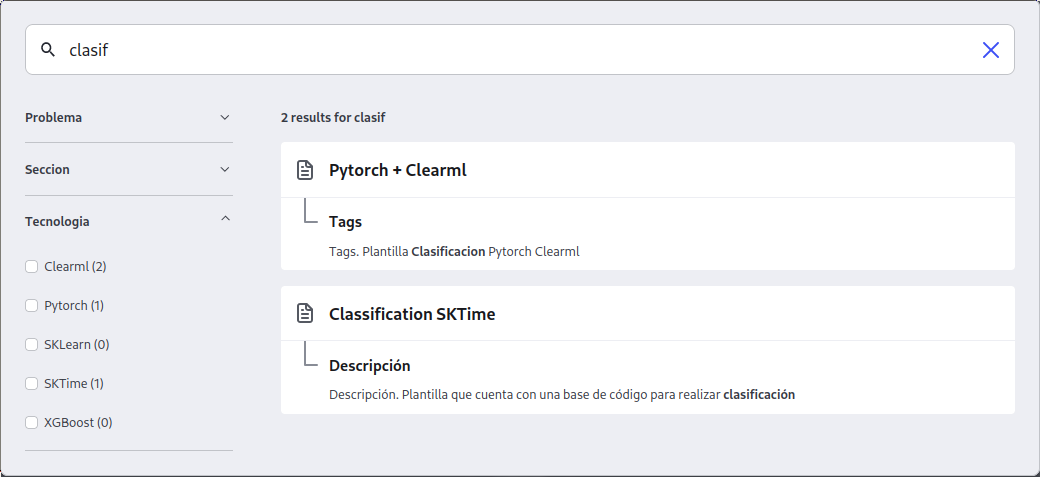
\includegraphics[width=0.85\textwidth]{search-menu.png}
    \caption{Sistema de búsqueda}\label{fig:search-menu}
\end{figure}

\subsubsection{Construcción automática de documentación}
Como se ha mencionado anteriormente, cada componente y plantilla 
viene con su propia documentación, la cual se genera dentro de su
respectiva carpeta mediante un archivo Readme.md. La decision de 
que cada componente tenga su documentación en su propia carpeta
es para facilitar la experiencia de desarrollo ya que todos los
elementos de cada componente se encuentran en un mismo lugar y no
es necesario buscar en diferentes carpetas para encontrar la
información necesaria.\medskip

Esto pese a ser una ventaja, también genera un problema a la hora de
generar la documentación, ya que es necesario un sistema que sea
capaz de recorrer todas las carpetas, extraer los archivos Readme.md
y Readme.mdx de cada una de ellas y generar la respectiva página
de documentación. Para solucionar este problema, se ha creado un
script de bash que recorre las carpetas que contienen componentes o
plantillas y copia estos archivos en una carpeta con el nombre de
su carpeta original con el fin de evitar problemas de colisiones
entre los nombres de los diferentes archivos. Una vez hecho esto,
se ejecuta el comando astro build y se sube la documentación a la
plataforma de GitLab Pages.



\pagebreak
    \section{Conclusiones y trabajo a futuro}
En esta sección se presentan las conclusiones obtenidas tras la finalización 
del proyecto, así como las lecciones aprendidas y los conocimientos adquiridos. 
Además, se presentan ideas o propuestas que podrían ser utilizadas o implementadas 
en el futuro para mejorar o ampliar el alcance del proyecto.

\subsection{Conclusiones}
Una vez finalizado el proyecto, se presentan las siguientes conclusiones en 
base a los resultados obtenidos y analizados durante el desarrollo del mismo.
Estas representan los cuatro aspectos clave del proyecto: reducción del tiempo de desarrollo, 
mejora de la productividad, reutilización del conocimiento y colaboración. Estas conclusiones 
reflejan los beneficios tangibles que el marco tecnológico propuesto aporta a los 
equipos y sus proyectos.\medskip

La implementación ha demostrado ser eficaz en la reducción significativa del tiempo 
de de\-sarro\-llo. Al automatizar tareas repetitivas y procesos manuales, se liberan 
recursos y se acelera el progreso de los proyectos. La adopción de metodologías 
ágiles y MLOps permite responder rápidamente a los cambios del entorno empresarial, 
proporcionando una ventaja competitiva crucial en cuanto a tiempo se refiere. La 
integración de plataformas como ClearML y Rath facilita la gestión y 
monitorización de experimentos, lo que reduce el tiempo dedicado a la configuración 
y gestión manual de estos procesos.\medskip

La mejora de la productividad es uno de los beneficios más destacados de la 
implementación del marco tecnológico. La automatización de tareas y la 
estandarización de procesos permiten a los equipos centrarse en actividades 
de mayor valor añadido. Además, el uso de herramientas de colaboración y la 
integración de sistemas de gestión del conocimiento aseguran que la información 
se comparta y reutilice de manera efectiva. Esto no solo incrementa la eficiencia 
operativa, sino que también mejora la calidad del trabajo, ya que los investigadores 
pueden dedicar más tiempo a la innovación y menos a tareas repetitivas.\medskip

El diseño de un sistema de componentes reutilizables y plantillas base para 
proyectos específicos facilita la reutilización del conocimiento adquirido. 
La creación de un catálogo de componentes esenciales y la documentación exhaustiva 
del proyecto aseguran que las mejores prácticas y soluciones previas se 
puedan aplicar en futuros proyectos. Este enfoque modular y estandarizado no 
solo ahorra tiempo, sino que también mejora la coherencia y calidad de los 
desarrollos, permitiendo a los equipos construir sobre trabajos anteriores 
de manera más eficiente.\medskip

La adopción de un marco común y la integración de herramientas colaborativas 
son fundamentales para mejorar la cooperación entre los miembros del equipo. 
La estandarización de procesos y la implementación de sistemas de autenticación 
y seguridad, como Keycloak, garantizan un entorno seguro y accesible para todos 
los miembros del equipo. Además, la encuesta de satisfacción realizada a los
miembros del equipo ha sido acogida de manera positiva, lo que sugiere que
existe un interés y una aceptación generalizada del nuevo marco tecnológico.\medskip

En conclusion, en base a los resultados obtenidos y analizados durante el desarrollo
del proyecto, se puede afirmar que la implementación del marco tecnológico propuesto
ha sido exitosa. Los beneficios tangibles obtenidos son muy positivos y sugieren que
el uso de este marco tecnológico puede mejorar significativamente la eficiencia y
productividad de los equipos.

\subsection{Trabajo a futuro}
A continuación, se presentan las siguientes propuestas de mejora y ampliación
del proyecto que podrían ser implementadas en futuras iteraciones:

\begin{itemize}
    \item \textbf{Adaptación del sistema a visión por computador:} Actualmente, la infraestructura 
    está enfocada en problemas basados en series temporales, pero se podría ampliar
    su alcance para incluir problemas de visión por computador. Se podría implementar
    no solo funcionalidades de preprocesamiento de imágenes, sino también incluir
    plataformas de etiquetado de imágenes populares como Cvat \cite{CVAT} o incluso conectar el
    sistema de versionado de datasets con herramientas como FiftyOne \cite{FiftyOne}.
    \item \textbf{Integración de ClearML con las tarjetas gráficas de la empresa:} Para 
    optimizar el uso de recursos de cómputo, se propone conectar ClearML con las 
    gráficas (GPUs) de la empresa. Esta integración permitirá gestionar y monitorear las 
    tareas de procesamiento de manera eficiente, asegurando una distribución adecuada de las 
    cargas de trabajo. ClearML facilitará la asignación dinámica de recursos, mejorando 
    la eficiencia del procesamiento y reduciendo tiempos de espera. Se podría implementar un 
    sistema de colas que divida las tareas según su prioridad y requerimientos de recursos. 
    Esto incluiría la creación de diferentes colas para tareas de alta prioridad, 
    tareas de procesamiento intensivo y tareas de mantenimiento. ClearML gestionaría estas colas, 
    asignando las tareas a las GPUs disponibles y asegurando un uso equilibrado y eficiente de los recursos.
    \item \textbf{Monitorización y análisis de rendimiento:} Implementar herramientas de monitorización 
    que proporcionen métricas detalladas sobre el uso de los recursos, el rendimiento de las 
    tareas y la eficiencia del sistema en general. Estas herramientas permitirían identificar 
    cuellos de botella, optimizar la asignación de recursos y planificar mejoras futuras 
    basadas en datos concretos. Además, se podría implementar un sistema de alertas que
    notifique sobre posibles problemas o anomalías en el rendimiento del sistema, permitiendo
    una respuesta rápida y eficaz ante situaciones críticas.
\end{itemize} 
    \pagebreak 
    \printbibliography[title=Bibliografía]
    \pagebreak
\end{document}